\documentclass[a4paper,9pt]{ctexart}

\usepackage{tikz}
\usepackage{circuitikz}
\usetikzlibrary{decorations.pathmorphing}

%\usepackage{fancyhdr}
\usepackage{amsmath,amssymb}
\usepackage{graphicx}
%\usepackage[hmargin=1.25in,vmargin=1in]{geometry}
\usepackage{pdfpages}
\usepackage[colorlinks,
            linkcolor=red,
		 urlcolor=purple]{hyperref}
\usepackage{cleveref}
\usepackage{float}

\crefname{equation}{}{}
\crefname{figure}{图}{图}
\crefname{footnote}{注释}{注释}
\crefname{table}{表}{表}

%\cpic{<尺寸>}{<文件名>}}用于生成居中的图片。
\newcommand{\cpic}[2]{
\begin{center}
\includegraphics[width=#1\textwidth]{#2}
\end{center}
}

%\cpicn{<尺寸>}{<文件名>}{<注释>}用于生成居中且带有注释的图片,其label为图片名。
\newcommand{\cpicn}[3]
{
\begin{figure}[H]
\cpic{#1}{#2}
\caption{#3\label{#2}}
\end{figure}
}

\newcommand{\beq}{\begin{equation}}
\newcommand{\eeq}{\end{equation}}
\newcommand{\bea}{\begin{equation}\begin{aligned}}
\newcommand{\eea}{\end{aligned}\end{equation}}

%输入单位和数学常数
%下面所有命令需在公式环境下使用
\newcommand{\e}{\mathrm{e}}   %自然常数e = \e
\newcommand{\im}{\mathrm{i}}   %虚数单位i = \im
\newcommand{\meter}{\mathrm{m}}      %单位/前缀 = \单位/前缀英文名
\newcommand{\newton}{\mathrm{N}}  
\newcommand{\joule}{\mathrm{J}}
\newcommand{\second}{\mathrm{s}}
\newcommand{\gram}{\mathrm{g}}
\newcommand{\ampere}{\mathrm{A}}
\newcommand{\kilo}{\mathrm{k}}
\newcommand{\milli}{\mathrm{m}}
\newcommand{\kelvin}{\mathrm{K}}
\newcommand{\mole}{\mathrm{mol}}
\newcommand{\volt}{\mathrm{V}}
\newcommand{\nano}{\mathrm{n}}
\newcommand{\degreeC}{^\circ \mathrm{C}}  %摄氏度符号 = \degreeC

\newcommand{\so}{ $\Rightarrow$ }
\newcommand{\info}[1]{{\bf \color{red} #1}}

\newcommand{\reals}{\mathbb{R}}
\newcommand{\complexs}{\mathbb{C}}
\newcommand{\ints}{\mathbb{Z}}
%\newcommand{\dim}{\mathrm{dim\ }}
\newcommand{\up}{\uparrow}
\newcommand{\down}{\downarrow}
\newcommand{\del}{\vec \nabla}
\newcommand{\su}{\mathfrak{su}}
\newcommand{\lbk}{\left(}
\newcommand{\rbk}{\right)}

\DeclareMathOperator{\tr}{tr}
\DeclareMathOperator{\diag}{diag}
\newcommand{\card}{\mathrm{card \ }}
\newcommand{\mani}{\mathcal{M}}
\newcommand{\lag}{\mathcal{L}}
\newcommand{\ham}{\mathcal{H}}
\def\secpage#1#2{\begin{frame}\bch\bcenter{\bf \Huge #1} \skipline \tbox{#2}\ecenter\ech\end{frame}}
\newcommand{\mat}[1]{\begin{pmatrix}#1\end{pmatrix}}
\newcommand{\mev}{\ {\rm MeV}}
\newcommand{\pfrac}[2]{\frac{\partial #1}{\partial #2}}

\newcommand{\unit}[1]{{\rm \ #1}}
\newcommand{\emptyline}{\par \ \\ }

\newtheorem{eg}{例}[section]
\newtheorem{ans}{解答}[section]


\def\bropt{\,(\ \ \ )}
\def\optlist#1#2#3{(A)\;#1\ \ \ (B)\;#2\ \ \ (C)\;#3}
\def\ooptlist#1#2#3#4{(A)\;#1\ \ \, (B)\;#2\ \, \ (C)\;#3\ \, (D)\;#4}

\newcommand{\emf}{{\cal E}}
\title{高中物理讲义\\ PART II: Electromagnetism}
\author{Han Gao\footnote{gaoh26@mail2.sysu.edu.cn}}
\begin{document}
\maketitle
\tableofcontents
\section{静电学}
(under construction...)
\section{直流电路}
(under construction...)
\section{静磁学}
(under construction...)
\newpage
\section{电磁感应}
\subsection{感生电动势和动生电动势}
\emph{法拉第最开始怎么发现的电磁感应现象?}
\begin{itemize}
\item
电磁感应定律
\beq
\emf = \frac{\Delta \Phi}{\Delta t}
\eeq
\item
$\Delta \Phi$是回路内磁通的\info{变化量}(和速度、加速度、电流等一样的数学),由两部分组成
\begin{enumerate}
\item
感生:由回路内的磁场增大导致,$\Delta \Phi = (\Delta B) S$ \so $\emf = S \frac{\Delta B}{\Delta t}$;
\item
动生:由回路面积变化导致,$\Delta \Phi = B \Delta S$ \so $\emf = Blv$。
\end{enumerate}
\item
如\cref{emf2kind},对应不同的物理:感生电动势对应“动磁生电”(选修3-4学习);动生电动势对应运动导线内电子受到的洛伦兹力(类似于霍尔效应)。 \so $\emf = \frac{\Delta \Phi}{\Delta t}$永远正确,而$\emf = Blv$只对恒定磁场适用(c.f. 2016年高考压轴题)。
\cpicn{0.8}{emf2kind}{感生电动势(左)和动生电动势(右)}
\item
动生电动势来源于洛伦兹力 \so 存在少许\emph{看似}没有磁通量变化,却也发生电磁感应的特例(阿拉果圆盘,某年全国卷高考题,如\cref{alago})。
\cpicn{0.6}{alago}{阿拉果圆盘,试判断图中感应电流的方向}
\end{itemize}
\begin{eg} \label{egphib}
如\cref{phib},两平行导轨间距为$h$。在$t=0$时刻杆从距回路左端$s$处开始以匀速$v$向右运动,左边的磁场长度为$l<s$,大小随时间变化,为$B_1 = kt + B_0$,方向向下;右边的磁场大小恒定为$B_2$,方向向上,求
\begin{enumerate}
\item
在$t$时刻通过回路的磁通量;
\item
若回路接负载$R$,求感应电动势和感应电流的大小。
\end{enumerate}
\end{eg}
\cpicn{0.6}{phib}{通过回路的磁通量是什么意思?}
\begin{ans}
取向上为正方向,则左边的磁场正向贡献磁通量,为$\Phi_1 = B_1 lh = (B_0 + kt) lh$;右边的磁场反向贡献磁通量,为$\Phi_2 = -B_2 (s+vt-l)h$。通过回路的总磁通量为
\beq
\Phi(t) = [(B_0 + kt) l -B_2 (s+vt-l)] h
\eeq
取任意的时间间隔$\Delta t$,根据电磁感应定律
\beq
\emf = \frac{\Phi(t+\Delta t) - \Phi(t)}{\Delta t} = (kl - B_2v)h
\eeq
感应电流的大小为$I = \frac{\emf}{R} = \frac{(kl-B_2v)h}{R}$
\end{ans}

\subsection{楞次定律、电磁阻尼和电感}
\emph{如果杆能一直在磁场中运动下去,岂不是制成了永动机?}
\begin{itemize}
\item
\info{楞次定律}:感应电流总是试图阻止磁通量的变化,也即总存在一个物理机制阻碍电磁感应的发生。
\item
具体体现:来拒去留、增缩减扩...... \so E.g. 固定的线圈内通过的磁场强度突然变大,则线圈会有收缩的趋势;回路中的杆切割磁感线运动,则安培力会企图使杆减速;......
\item
是能量守恒定律在电磁感应中的体现! \so 更广泛的自然思想:负反馈调节机制;勒夏特列原理。
\item
\info{右手定则}判断感应电流的方向(是楞次定律在动生情况下的特例)。

\end{itemize}
\begin{eg}
一个线圈正上方悬挂了一个磁铁,将悬挂磁铁的线剪断,磁铁下落的加速度$a$与重力加速度$g$的大小关系是什么?
\end{eg}
\begin{ans}
总有物理机制会阻碍电磁感应顺利地发生,即阻碍磁铁下落,因此\uline{\hspace{4cm}}。
\end{ans}
\begin{itemize}
\item
在这个例子中,如果线圈是超导体,则磁铁可以一直悬空! \so 超导磁悬浮原理。
\end{itemize}
\begin{eg}
\cref{lenzlaw}是一个演示楞次定律的小玩具,线圈上平放的环是金属导体制成的。当开关接通电源时,你期待看到什么现象?为什么?
\end{eg}
\cpicn{0.6}{lenzlaw}{一个演示楞次定律的小玩具}
\begin{ans}
接通电源时下面的线圈内会产生磁场,使得通过金属环的磁通量增大,而楞次定律保证了存在一个物理机制来阻碍这个磁通量增大,因此\uline{\hspace{2cm}}
\end{ans}
\begin{eg}
在\cref{phib}中,杆受到的安培力朝什么方向,感应电流朝什么方向(需要分类讨论)?
\end{eg}
\begin{ans}
若$kl>B_2 v$,通过回路的磁通量在增大,于是安培力会想让这个磁通量减小,于是\uline{\hspace{6cm}}。
\vspace{5cm}
\end{ans}
\par
\emph{为什么地铁列车进站停车时几乎听不到刹车声音?这个减速过程是通过什么物理原理实现的?}
\begin{itemize}
\item
\info{电磁阻尼}:导体进入磁场区域时,由于切割磁感线运动发生电磁感应 \so 楞次定律保证了存在物理机制阻碍这样的运动,如\cref{emdamp}。
\item
\info{涡电流}:发生电磁阻尼现象时,导体内的电流,如\cref{emdamp}。
\cpicn{0.6}{emdamp}{电磁阻尼现象和涡电流}
\item
电磁阻尼现象的能量转换:机械能 $\to$ 电能 $\to$ 热能。
\item
如果能够减少"电能 $\to$ 热能"一步的转换,则可以减少能量损耗 \so 地铁列车、动车进站减速时利用电磁感应补充少许电能。
\end{itemize}
\par
\emph{将一个线圈接在直流电路中,把开关断开的一瞬间,为什么可以在开关的刀口处看见电火花?}
\begin{itemize}
\item
一个金属线圈自然地构成了一个\info{电感}。
\item
线圈通电时内部存在磁通量,断开时磁通量减小到0;而楞次定律阻碍了这个磁通量减小 \so 电感线圈会试图在短时间内维持电流使得磁通量缓慢减小,如\cref{rlcir}。
\cpicn{0.6}{rlcir}{电路断开开关后,存在电感的电路(实线)和无电感电路(虚线)的电流变化}
\item
理解:广义的惯性,电感赋予电路维持自身状态的能力。电感系数用$L$表示,决定因素:匝数、有无铁芯、线圈长度和宽度(和电磁铁磁性的决定因素一样)。
\end{itemize}
 
\subsection{电磁感应中的动力学问题}
\emph{如果题目不问,你需要先判断感应电流方向,再判断安培力方向吗?}
\begin{itemize}
\item
对动生问题,$\emf = Blv$可以有效解决,常见推论:
\beq
I = \frac{Blv}{R},\quad F = \frac{B^2 l^2 v}{R},\quad P = \frac{(Blv)^2}{R}
\eeq
\item
楞次定律保证物理机制阻碍电磁感应现象 \so 安培力总是阻力。
\item
这里的$l$应该理解为切割磁感线的有效长度。
\end{itemize}
\newpage
\begin{eg} \label{em2020}
【2020全国3卷】如\cref{20203},一边长为$l_0$的正方形金属框$abcd$固定在水平面内,空间内存在方向垂直于水平面,磁感应强度为$B$的匀强磁场,一长度大于$\sqrt 2 l_0$的均匀导体棒以速率$v$自左向右在金属框上匀速滑过,滑动过程中导体棒始终与$ac$垂直且中点位于$ac$上,导体棒与金属框接触良好。已知导体棒单位长度的电阻为$r$,金属框电阻可忽略。将导体棒与$a$点之间的距离记为$x$,求导体棒所受安培力大小随$x(0\leq x \leq \sqrt 2 l_0)$变化的关系式。
\end{eg}
\begin{figure}[H]
\centering
\begin{tikzpicture}
\draw (0,0) node[left]{$a$} -- (2,2) node[above]{$b$} -- (4,0) node[right]{$c$} -- (2,-2) node[below]{$d$} -- node[left]{$l_0$}  cycle ;
\draw (1,2) -- node[left]{$r$} (1,-2) ;
\draw[dotted] (0,0) -- (4,0);
\end{tikzpicture}
\caption{\cref{em2020}图\label{20203}}
\end{figure}
\begin{ans}
\ \\
\vspace{6cm}
\end{ans}
\newpage
\par
\emph{楞次定律保证了电磁感应过程中的能量守恒,这个能量守恒是怎么定量体现的?}
\begin{itemize}
\item
电磁感应需要外力维持,外力总是做正功。
\item
如果不存在摩擦力,外力功率=安培力做功功率=电阻(负载)消耗功率;如果存在摩擦损耗,则外力功率会更大(能量守恒角度理解)。
\end{itemize}
\begin{eg} \label{em2014}
【2014全国2卷】半径分别为$r$和$2r$的同心圆形导轨固定在同一水平面内,一长为$r$、质量为$m$且质量分布均匀的直导体棒$AB$置于圆导轨上面,$BA$的延长线通过圆导轨中心$O$,装置的俯视图如\cref{20142}所示。整个装置位于一匀强磁场中,磁感应强度的大小为$B$,方向竖直向下。在内圆导轨的$C$点和外圆导轨的$D$点之间接有一阻值为$R$的电阻(图中未画出)。直导体棒在水平外力作用下以角速度$\omega$绕$O$逆时针匀速转动,在转动过程中始终与导轨保持良好接触。设导体棒与导轨之间的动摩擦因数为$\mu$,导体棒和导轨的电阻均可忽略。重力加速度大小为$g$。求
\begin{enumerate}
\item
通过电阻$R$的感应电流的方向和大小;
\item
外力的功率。
\end{enumerate}
\end{eg}
\begin{figure}[H]
\centering
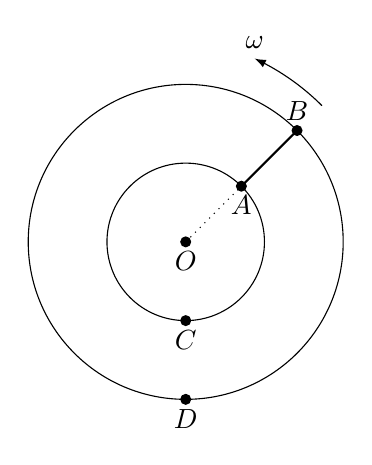
\begin{tikzpicture}
\draw (0,0) circle [radius=1];
\draw (0,0) circle [radius =2];
\fill (0,0) circle [radius = 2pt];
\fill (0.707,0.707) circle [radius = 2pt];
\fill (1.414,1.414) circle [radius = 2pt];
\fill (0,-1) circle [radius = 2pt] node[below]{$C$};
\fill (0,-2) circle [radius = 2pt] node[below]{$D$};
\draw[dotted] (0,0) node[below]{$O$} -- (0.707,0.707) node[below]{$A$};
\draw[thick] (0.707,0.707) -- (1.414,1.414) node[above]{$B$};
%\draw[-latex] (2,1.5) -- node[right]{$\omega$} (1.5,2);
\draw[-latex] (1.73,1.73) arc(45:65:3) node[above]{$\omega$} ;
\end{tikzpicture}
\caption{\cref{em2014}图\label{20142}}
\end{figure}
\begin{ans}
(在这种情况下,还能用$\emf = Blv$计算动生电动势吗?)
\vspace{8cm}
\end{ans}
\newpage
\par
\emph{同时存在动生电动势和感生电动势,应该用哪个公式计算$\emf$?}
\begin{eg} \label{em2016}
【2016全国3卷】如\cref{20163},两条相距$l$的光滑平行金属导轨位于同一水平面(纸面)内,其左端接一阻值为$R$的电阻;一与导轨垂直的金属棒置于两导轨上;在电阻、导轨和金属棒中间有一面积为$S$的区域,区域内存在垂直于纸面向里的均匀磁场,磁感应强度大小$B_1$随时间的变化关系为$B_1 = kt$,式中$k$为常量;在金属棒右侧还有一匀强磁场区域,区域左边界$MN$(虚线)与导轨垂直,磁场的磁感应强度大小为$B_0$,方向也垂直纸面向里。某时刻,金属棒在一外加水平恒力的作用下从静止开始向右运动,在$t_0$时刻恰好以$v_0$速度越过$MN$,此后向右做匀速运动。金属棒与导轨始终相互垂直并接触良好,它们的电阻均忽略不计。求
\begin{enumerate}
\item
在$t=0$到$t=t_0$时间间隔内,流过电阻电荷量的绝对值;
\item
在时刻$t(t>t_0)$穿过回路的总磁通量和金属棒所受外加水平恒力的大小。
\end{enumerate}
\end{eg}
\cpicn{0.6}{20163}{\cref{em2016}图}
\begin{ans}
\ \\
\vspace{8cm}
\end{ans}
\newpage
\par
\emph{如果电路上接的不是电阻是电容,这题还能做吗?}
\begin{itemize}
\item
电容上的电荷量与电压的关系$q = CU$ \so 两边取变化率,利用$I = \frac{\Delta q}{\Delta t}$ \so $I = C \frac{\Delta U}{\Delta t}$。
\item
如果切割磁感线的是平行杆,$U = \emf = Blv$ \so 两边取变化率,利用$a = \frac{\Delta v}{\Delta t}$ \so $ \frac{\Delta U}{\Delta t} = Bla$。
\item
选修3-1书上直流电流的定义式$I = q/t$一定要理解成$I = \Delta q /\Delta t$!
\item
$\frac{\Delta (\dots)}{\Delta t}$的含义是对时间求导...
\item
灵活变通,高考总不可能永远考同一个模型,那就人人满分了... \so 真正地理解物理!
\end{itemize}
\begin{eg} \label{em2013}
【2013全国1卷】如\cref{20131},两条平行导轨所在平面与水平地面的夹角为$\theta$,间距为$L$。导轨上端接有一平行板电容器,电容为$C$。导轨处于匀强磁场中,磁感应强度大小为$B$,方向垂直于导轨平面。在导轨上放置一质量为$m$对金属棒,棒可沿导轨下滑,且在下滑过程中保持与导轨垂直并良好接触。已知金属棒与导轨之间的动摩擦因数为$\mu$,重力加速度大小为$g$。忽略所有电阻。让金属棒从导轨上端由静止开始下滑,求:
\begin{enumerate}
\item
电容器极板上积累的电荷量与金属棒速度大小的关系;
\item
金属棒的速度大小随时间变化的关系。
\end{enumerate}
\end{eg}
\cpicn{0.6}{20131}{\cref{em2013}图}
\begin{ans}
\ \\
\vspace{8cm}
\end{ans}
\section{交流电路}
\subsection{交流发电机与正弦交流电的描述}
\emph{\cref{egene}中,哪个是直流发电机,哪个是交流发电机?}
\cpicn{0.8}{egene}{发电机}
\begin{itemize}
\item
交流发电机:线圈在匀强磁场中沿垂直磁场的轴转动 \so 磁通量变化产生电动势。
\item
电动势大小:考虑单匝线圈,$\emf = 2Bl_1 v\sin \omega t =BS\omega \sin \omega t$,如\cref{acgen}。
\item
另一种想法:磁通量$\Phi = BS\cos \omega t$,两边对时间求导:$\emf = -\frac{d\Phi}{dt} = BS \omega \sin \omega t$。
\begin{figure}[H]
\centering
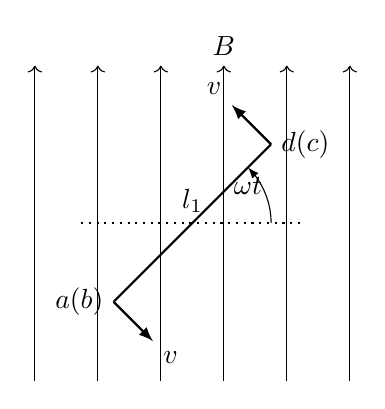
\begin{tikzpicture}
\draw[->] (0,-2) -- (0,2);
\draw[->] (0.8,-2) -- (0.8,2);
\draw[->] (1.6,-2) -- (1.6,2);
\draw[->] (2.4,-2) -- (2.4,2)node[above]{$B$};
\draw[->] (3.2,-2) -- (3.2,2);
\draw[->] (4,-2) -- (4,2) ;
\draw[-latex,thick] (1,-1) -- (1.5,-1.5) node[below right]{$v$};
\draw[-latex,thick] (3,1) -- (2.5,1.5) node[above left]{$v$};
\draw[thick] (1,-1) node[left]{$a(b)$}-- node[above]{$l_1$} (3,1) node[right]{$d(c)$};
\draw[dotted,thick] (0.586,0) -- (3.414,0);
\draw[-latex] (3,0) arc(0:45:1)  node[below]{$\omega t$};
\end{tikzpicture}
\caption{交流发电机的磁通量\label{acgen}}
\end{figure}
\item
磁通量最大的面称为\info{中性面},该点$\emf=0$。
\item
$N$匝线圈同时发电:$\emf = NBS\omega \sin \omega t$。
\item
正弦交流电:电压$u = U_m \sin \omega t$,电流$i = I_m \sin \omega t$。
\item
jargon:$U_m,I_m$电压(电流)最大值(或称峰值);$\omega$称为角频率;$f = \frac{\omega}{2\pi}$称为频率;$T = \frac{2\pi}{\omega}$称为周期(请复习数学三角函数知识)。
\item
中国\info{市电}:$U_m = 220\sqrt 2 \unit V \approx 311\unit V$,$f = 50\unit{Hz}$,$T = 0.02\unit s$;在美国等一些国家$U_m = 110\sqrt 2 \unit V$;还有一些加拿大等少数西方国家用$f = 60\unit{Hz}$(为什么出国旅游要带电压转换器的原因)。
\end{itemize}

\subsection{有效值、变压器和高压输电}
\emph{我们平时说的$220\unit V$交流电是指什么意思?正弦交流电的电压在一个周期内的平均值是多少?}
\begin{itemize}
\item
交流电(AC):大小和方向都随时间变化的电流;直流电(DC):方向不随时间变化的电流 \so DC的大小可以随时间变化...
\item
交流电的有效值定义为:
\begin{enumerate}
\item
物理:若交流电$i$在一个周期$T$内通过一个电阻$R$,产生的热量为$Q$,则其有效值为使得同样的电阻在$T$时间内产生同样热量的直流电流的大小,即$I_{\rm rms} = \sqrt{\frac{Q}{RT}}$。
\item
数学:周期函数$i(t)$的有效值(又称方均根,root mean square)是周期函数$i(t)$在一个周期内\info{平方的平均值开根号}。如果你已经在《数学:选修2-2》里学了积分,就是
\beq \label{rmsdef}
I_{rms} = \sqrt{\frac{\int_0^T i^2(t)dt}{T}}
\eeq
\end{enumerate}
\item
物理定义和数学定义是严格等价的。
\item
可以利用\cref{rmsdef}得到正弦交流电的有效值$U_{rms}$和$U_m$之间的关系为
\beq
U_m = \sqrt{2} U_{rms}
\eeq
\item
对更一般的时变电流(电压)计算有效值:先求平方平均,再开根号。
\end{itemize}
\begin{eg}
如\cref{waveform}是一个交流电压$u$在一个周期$T$内的图像,在$0-0.5T$内为一段完整的正弦图像,峰值为$2\unit V$;$0.5T-0.8T$内是一段电压为$-1\unit V$的恒定电压;$0.8T-1T$内是一段电压为$3\unit V$的恒定电压。求这个交流电压的有效值。
\end{eg}
\cpicn{0.6}{waveform}{一个奇怪的交流电波形}
\begin{ans}
在$0-0.5T$内,这个正弦信号的有效值为$\sqrt 2\unit V$,因此其平方在这段时间的累积为$(\sqrt 2 )^2\times 0.5 T = T$;后两段信号的平方累积分别为$0.3T$和$1.8T$。因此有效值为
\beq
U_{rms} =\sqrt{ \frac{\sum_{\text{各时间段}} U^2 \Delta t}{T}}= \sqrt{4.1}\unit V
\eeq
\end{ans}

\subsection{变压器}
\emph{电气历史前期一直有到底是应用直流(爱迪生为代表)还是交流(特斯拉为代表)的争论。为什么交流电最终赢得了胜利?}
\begin{itemize}
\item
交流电的好处:可以及其方便地转换电压。
\item
变压器:两个匝数分别为$n_1$和$n_2$的线圈缠绕在一起,流过的磁通相等(无漏磁) \so 电磁感应定律给出
\beq
\frac{U_1}{U_2} = \frac{n_1}{n_2}
\eeq
$U_{1,2}$是交流电压的有效值。
\item
\cref{transformer}是一种输出电压可变的变压器。
\cpicn{0.6}{transformer}{一种输出电压可变的变压器}
\item
理想变压器:无漏磁且无能量损耗,两端消耗的电功率相等 \so $U_1 I_1 = U_2 I_2$ \so $n_1 I_1 = n_2 I_2$。
\item
应用:电流检测器:小的$n_1$接在待测的载流输电线上;大的$n_2$接电流表 \so 得到输电线上的电流。
\end{itemize}

\subsection{高压输电}
\emph{高压输电的好处是在导线上的能量损耗小,但$P=U^2/R$,为什么不是$U$越大$P$越大呢?}
\begin{itemize}
\item
电压=电势差。电压都是针对两点定义的。 \so 单独提一根导线上的电压是指这根导线的对地电压。
\item
$P=U^2/R$中的$U$应该指导线两端的电压降而非对地电压(一般在这里我们更喜欢写成$\Delta U$表示电厂端到用户端的电压降)。但$P=I^2 R$作为\info{焦耳定律}是一个普适定律,总是适用的。
\item
理想变压器两端的功率相等 \so 提高输电电压减小了输电电流 \so 能量损耗减小。
\end{itemize}
\begin{eg}
如\cref{hvolteg},发电厂以$P_0$的功率输出$220\unit V$的交流电,经过变压器$T_1$后升压为$55\unit{kV}$。再经过输电线通向变压器$T_2$降压后输出给用户。当用户使用功率为$P=0.8P_0$时,用户接受到的电压恰好为$220\unit V$。求
\begin{enumerate}
\item
$P = 0.8P_0$且$P_0 = 110\unit{kW}$时,输电线上的功率损耗和电压降、电流。
\item
$T_1$和$T_2$的匝数比。
\item
当用户使用功率$P = 1.25P_0$时,用户接受到的实际电压仍然为$220\unit V$,求电厂需要输出的实际功率。
\end{enumerate}
\end{eg}
\begin{figure}[H]
\centering
\begin{circuitikz}
\draw (0,1.5) to[short,o-]  (0,2)
to[short](1,2)
to[L](1,0)
to[short](0,0)
to[short,-o](0,0.5);
\draw[very thick] (1.5,2)node[above]{$T_1$} --  (1.5,0);
\draw (2,0) to[L](2,2) to[short] (4,2) to[L] (4,0) to[short](2,0);
\draw[very thick] (4.5,2) node[above]{$T_2$} -- (4.5,0);
\draw (6,0.5) to[short,o-] (6,0) to[short] (5,0) to[L] (5,2) to[short] (6,2) to[short,-o] (6,1.5);
\begin{scope}[decoration={snake,amplitude=1mm,
        segment length=2.5mm}]
\draw[decorate] (-0.5,1) node[left]{$220\unit V, P_0$} -- (0.5,1);
\draw[decorate] (5.5,1)  -- (6.5,1) node[right]{$220\unit V, 0.8 P_0$};
\end{scope}
\end{circuitikz}
\caption{高压输电\label{hvolteg}}
\end{figure}
\begin{ans}
\begin{enumerate}
\item
由于$T_1,T_2$都是理想变压器,功率损耗仅发生在输电线上,为$\Delta P = P_0-P = 0.2P_0 = 22\unit{kW}$。又输电线上的电流为$I_1 = P_0/U_1 = 110\unit{kW} / 55\unit{kV} = 2\unit A$;其电压降为$\Delta U = \Delta P/I = 11\unit{kV}$。
\item
\ \\
\vspace{2cm}
\item
\ \\
\vspace{2cm}
\end{enumerate}
\end{ans}



\subsection{交流电路中的电感和电容}
\emph{美国的交流电是$110\unit V,50 \unit{Hz}$;而加拿大是$110\unit V,60\unit{Hz}$。假如发生触电事故,一般情况下哪国人受伤更严重?}
\begin{itemize}
\item
交流电路元件的电抗(阻抗)$X$定义为元件两端电压有效值和电流有效值之比。
\item
对电阻$X=R$,对电感$X = \omega L$,对电容$X = \frac{1}{\omega C}$。
\item
直流电可以看成$\omega = 0$的交流电 \so 电感频率越高阻抗越大(隔交阻直);电容频率越高阻抗越小(隔直阻交)。
\item
实际应用:滤波器,如\cref{filter},如果输入的电源信号$u(t)$同时包含直流和交流成分,则交流成分会通过电容;而直流成分会通过电感。
\end{itemize}
\begin{figure}[H]
\centering
\begin{circuitikz}
\draw (0,1.5) node[below]{{$u(t)$}} to[short,o-] (0,2) to[short] (2,2) to[C,C=$C$] (2,0) to [short] (0,0) to[short,-o] (0,0.5) ;
\draw (2,2) to[short] (4,2) to[L,L=$L$] (4,0) to[short] (2,0);
\end{circuitikz}
\caption{一个简单的滤波器电路\label{filter}}
\end{figure}









































\end{document}